\documentclass{article}
\usepackage[utf8]{inputenc}
\usepackage[linguistics]{forest}
\usepackage{clrscode3e}
\usepackage{mathtools}
\DeclarePairedDelimiter\ceil{\lceil}{\rceil}
\DeclarePairedDelimiter\floor{\lfloor}{\rfloor}

\title{Problem Set N° 2 - CS2102}
\author{Roosevelt J. Ubaldo}
\date{\today}

\begin{document}

\maketitle

\section*{Problem 1 (Cache oblivious median finding)}
Given an un-ordered array of N elements, develop and analyze a cache-oblivious algorithm to find the median of the array in $O(N/B)$ memory transfers. In your solution, you may assume knowledge of the standard median-of-median deterministic selection algorithm.

\noindent \textbf{Answer: }

\noindent Given an array $A$ of $n$ elements: 
\begin{codebox}
\Procname{$\proc{MedianFinding}(A)$}
\li Conceptually divide the n elements into groups of length 5 
\li Find the \proc{Median} of each subset
\li Recursively find the \proc{Median} $x$ of the groups of medians
\li Partition array by $x$
\li Recurse on one side
\li \Do \If $k$ ==  $\ceil{n/2}$ \Return $x$ \Comment where $k$ is the rank of $x$ \End
\li \Do \If $k < \ceil{n/2}$ \Return $\proc{MedianFinding}(A[0, \cdot, k-1])$ \End
\li \Do \If $k > \ceil{n/2}$ \Return $\proc{MedianFinding}(A[k+1, \cdot, n])$ \End
\end{codebox}

This procedure give us the following recursion: 
$$T(n) = n + T(\frac{n}{5}) + T(\frac{7n}{10})$$

However, we are going to analyze the cache oblivious of the aforementioned algorithm line by line:

\begin{enumerate}
    \item This step does not need any memory transfer because is just conceptual
    \item Assuming that the cache can holds two blocks at a time, one to read five elements of the array and other, in parallel, to write the computed median of the groups of five. This step uses $\Theta(N/B +1)$ memory transfers.
    \item This step is a recursive call of size $\ceil{N/5}$, the median of medians. 
    \item This step can be done with three parallel scans, one to read the array and the others for the partitions. This step uses $\Theta (N/B+1)$ memory transfers.
    \item This is a recursive call of at most $\frac{7}{10}N$ size.
\end{enumerate}

\noindent Therefore, the recurrence on the number of memory transfer will be:

$$MT(N) = MT\left(\frac{N}{5}\right)+ MT \left(\frac{7}{10}N\right) + O\left(\frac{N}{B}+1\right)$$

\noindent Assuming that $MT(1)=O(1)$ and  $MT(N) \geq L(N)$ where $L(N)$ is the number of leaves in the recursion, this satisfy the following equation:

$$L(N) = L\left(\frac{N}{5}\right) + L\left(\frac{7}{10}N\right)$$

This solves to some $N^\alpha$, so now the equation will turn like this:

\begin{align*}
    N^\alpha &= \left(\frac{N}{5}\right)^\alpha + \left(\frac{7}{10} N\right)^\alpha \\
    N^\alpha &=\left( \frac{1}{5}^\alpha + \frac{7}{10}^\alpha\right)N^\alpha \\
    1 &=\frac{1}{5}^\alpha + \frac{7}{10}^\alpha \\
    \alpha & \cong 0.83978 \\
    L(N) &\geq N^{0.8}
\end{align*}


As we might know this is not a good base case. However, if we chosse $MT(B) =O(1)$, then the number of leaves would be $\left(\frac{N}{B}\right)^\alpha = O\left(\frac{N}{B}\right)$, and as $O\left(\frac{N}{B} +1\right)$ is dominant the solution for this recursion will be $MT(N) = O\left(\frac{N}{B} +1\right)$

\section*{Problem 2 (Cache oblivious queue)}

Develop and analyze a cache-oblivious FIFO queue.  Both the enqueue and the dequeue operation should take $O(1/B)$ amortized memory transfers.  Your data structure should only use external memory indices in $0,1,...,O(N)$, where $N$ is the maximum number of elements store in the queue at once.

\textbf{Answer:}

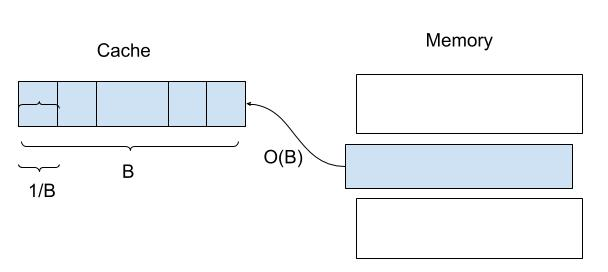
\includegraphics[scale = .5]{ej2.jpg}

\noindent As we read data from memory in blocks of length B, the first time that we insert an item to the queue we need to read the whole block and this will cost $O(B)$. However, if we want to insert another item, the cost of this operation will be "free" until we reach the final of the block (when we need to read another block), because we already read it in the previous operation. This is how the amortized cost of insert an item will be $O(1/B)$. The same logic applies to the dequeue operations. 


\section*{Problem 3 (Cache oblivious matrix multiplication)}

Describe the cache-efficient algorithm for computing the matrix product
$$C_{n \times n} = X_{n \times n} \times Y_{n \times n}$$
for parameters M and B.

\textbf{Answer:}

The matrix multiplication can be written as a divide and conquer recursion using block-matrix notation:

$$\begin{pmatrix}
A_{11} & A_{12} \\
A_{21} & A_{22} 
\end{pmatrix}
\begin{pmatrix}
B_{11} & B_{12} \\
B_{21} & B_{22}
\end{pmatrix} = 
\begin{pmatrix}
A_{11}B_{11} + A_{12}B_{21} & A_{11}B_{12}+A_{12}B_{22} \\
A_{21}B_{11} + A_{22}B_{21} & A_{21}B_{12} + A_{22}B_{22}
\end{pmatrix}$$

This is how the $N\times N$ matrix multiplication is reduced to $(\frac{N}{2})\times (\frac{N}{2})$ sub-matrix multiplications. Then, there are four sub-matrix additions that can be solved by a single scan in $O(1 + \frac{N^2}{B})$. Therefore, this algorithm has the following recurrence:

$$T(N) = 8T(N/2) + O\left(1+\frac{N^2}{B}\right)$$

Then we chose $MT(\sqrt{M/3}) = O(M/B)$ as base case because in this way we can fit in cache the three matrix involved together. Therefore, the recursion three will be:

\begin{forest}
[$\frac{N^2}{B}$[$\frac{N^2}{2^2B}$
[$\frac{N^2}{4^2B}$] [...] [$\frac{N^2}{4^2B}$] ][$\frac{N^2}{2^2B}$[$\frac{N^2}{4^2B}$] [...] [$\frac{N^2}{4^2B}$]][...][$\frac{N^2}{2^2B}$
[$\frac{N^2}{4^2B}$] [...] [$\frac{N^2}{4^2B}$] ][$\frac{N^2}{2^2B}$
[$\frac{N^2}{4^2B}$] [...] [$\frac{N^2}{4^2B}$]]]
\end{forest}

\bigbreak
The cost at each level will be $\frac{N^2}{B}$, $8\frac{N^2}{2^2B}$, $8^2\frac{N^2}{4^2B}$, .... Thus, the total cost will be:
$$MT(N)=O(M/B)\cdot8^{O(\lg N/ \sqrt{M})} = O\left(\frac{M}{B}\right)\cdot O\left(\left(\frac{N}{\sqrt{M}}\right)^3\right) = O \left(\frac{N^3}{B\sqrt{M}}\right)$$

\section*{Problem 4 (Cache oblivious priority queue)}

Describe an external memory priority queue data structure. This must support the operations delete-min, insert and delete efficiently. Use this to implement an external memory heap sort. The reader will have devise fast amortized version of the priority queue operations to make heapsort match the performance of the external memory merge sort since a straightforward application of n delete-min operations would result in an $O(n lgB(n/B))$ IOs.

\textbf{Answer:}




\section*{Problem 5 (Parallel disk model)}

Consider  a  realistic  extension  of  the  external  memory  model  where  there  are $D$ disks capable of simultaneous input and output.  That is, during any read operation, block of size $B$ can be read in parallel form each of the $D$ disks and similarly,$D$ blocks of size $B$ can be written in parallel.  This is more constrained compared to the ability of simultaneously accessing any set of $D$ block from a disk – which yields a virtual block size $DB$.

\begin{enumerate}
    \item Design an algorithm to transpose an $N\times N$ matrix that is faster that the single disk model.
    \item  Re-design the merge sort algorithm to exploit this $D$ fold increase in $IO$ capacity
\end{enumerate}

\textbf{Answer:}

\section*{Problem 6 (Cache oblivious matrix transpose)}

Design a cache-oblivious algorithm for computing matrix transpose for the case $M\geq B^{3/2}$. Recall that the method described in the chapter assumes that $M\geq B^2$

\textbf{Answer:}

In the transpose of a matrix $A_{m\times n}$ we change the rows of $A$ into the columns of a matrix $B_{n\times m}$.


$$A = \begin{pmatrix}
A_{11} & A_{12} \\
A_{21} & A_{22} \\
A_{31} & A_{23} 
\end{pmatrix}, C = A^T = \begin{pmatrix}
A_{11} & A_{21} & A_{31}\\
A_{12} & A_{22} & A_{32}
\end{pmatrix}$$

The pseudocode of a Naive Matrix Transpose is the following: 
\begin{codebox}
\Procname{$\proc{MatrixTranspose}(A)$}
\li \For $i=1$ to $m$ \Do
\li \For $j=1$ to $n$ \Do
\li $C_{ij} = A_{ji}$ \End\End
\li \Return C
\end{codebox}

In the cache oblivious matrix transpose algorithm we have the following cases: when the rows of the matrix fits into the cache block and when not. If is in the case one, we just transpose each element of the block and the memory transfers will be $MT(N^2/B +1)$. However, in the second case we need to divide the matrix by columns in order to fit into the cache block. The resultant algorithm will be:

\begin{codebox}
\Procname{$\proc{CacheObliviousMatrixTranspose}(A)$}
\li \If $\max(m,n) \leq B$ \Do
\li \Return $\proc{MatrixTranspose}(A)$ \End
\li \Else \If $n>m$ \Do
\li Divide $A$ into $A1_{m\times n/2}$ and $A2_{m \times n/2}$ 
\li $\proc{MatrixTranspose}(A1)$ 
\li $\proc{MatrixTranspose}(A2)$ 
\li \Else
\li Divide $A$ into $A1_{m/2\times n}$ and $A2_{m/2 \times n}$ 
\li $\proc{MatrixTranspose}(A1)$ 
\li $\proc{MatrixTranspose}(A2)$ 
\end{codebox}


\section*{Problem 7 (Parallel prefix-sum)}

Develop the parallel prefix-sum in an iterative way (without recursion). The algorithm shoul work $O(n)$ and paralism $\Theta(n/ \lg n)$

\textbf{Answer: }

First of all, we are going to write the pseudocode of the iterative prefix sum: 
\begin{codebox}
\Procname{$\proc{IterativePrefixSum}(A)$}
\li \For $i = 1$ to $n -1$ \Do
\li $A[i]=A[i-1] + A[i]$ \End
\li \Return A
\end{codebox}

As the value of $B[i]$ depends of the value of  $B[i-1]$ seems to be difficult to generate a parallel algorithm. However as the result of this algorithm is a cumulative sum, we can treat this algorithm as a sum of little cumulative sums. For the following parallel algorithm we assume that $n$ is a power of $2$

\begin{center}
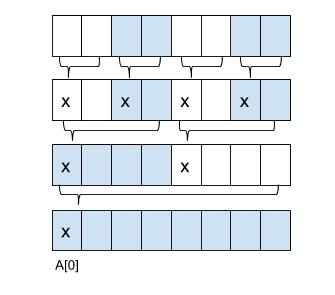
\includegraphics[scale=.5]{ej7.jpg} 
\end{center}

\begin{codebox}
\Procname{$\proc{ParallelIterativePrefixSum}(A)$}
\li \For $i = 1$ to $n -1$ \Do
\li size = $n/(2\times i)$
\li $k = i$
\li \For $j= 0$ to size $- 1$ \Do
\li $A[2\times j \times k]+= A[(2\times j+1)\times k]$ \End 
\li $i = i \times 2$ \End
\li \Return A[0]
\end{codebox}


\section*{Problem 8 (Parallel Quick-sort)}

Develop the parallel quick-sort algorithms. The algorithm should work $O(n \lg n)$for average case and parallelism $\Theta(n/lgn)$.

\textbf{Answer:}

First of all, we write the pseudocode of $\proc{QuickSort}$
\begin{codebox}
\Procname{$\proc{QuickSort}(A,l,r)$}
\li \If $(l<r)$ \Do
\li $q = \proc{Partition}(A, l, r)$
\li $\proc{QuickSort}(A,l, q)$
\li $\proc{QuickSort}(A,q+1, r)$
\end{codebox}

This pseudocode give as the recurrence $T(N) = 2 T(N/2) + O(n)$ for one processor, an it solution will be $O(n)$. However in the parallel analysis we assume that we have infinite processors $T_{\infty}= T(N/2) +O(n)$, so the solution will be $O(n\log n)$. 

\begin{codebox}
\Procname{$\proc{QuickSortParallel}(A[0:n/p],l,r)$}
\li \If $(l<r)$ \Do
\li $q = \proc{Partition}(A[0:n/p], l, r)$
\li $\proc{QuickSort}(A[0:n/p],l, q)$
\li $\proc{QuickSort}(A[0:n/p],q+1, r)$ \End
\li \proc{JoinResult}
\end{codebox}
\section*{Problem 9 (Parallel multidimensional-sort)}

Consider the following algorithms to sort an $n\times n$ array of numbers.  Assume for simplicity that $n=2^k$.

\begin{itemize}
    \item Sort the four $\frac{n}{2} \times \frac{n}{2}$ sub-arrays recursively according to some indexing scheme.
    
    \textbf{Answer:}
    
    \item Prove that algorithm correctly sorts and analyze the parallel running time.
    
    \textbf{Answer:}
\end{itemize}

\section*{Problem 10 (Parallel Merge-sort)}

In this problem we will improve the parallel merge-sort algorithms from lecture.   The algorithm described in class has work $\Theta(n lgn)$.  and parallelism $\Theta(n/lg2n)$.  We should develop an algorithms with the same work, but higher parallelism.

\begin{itemize}
    \item Given two sorted arrays containing a total of $n$ elements, give an algorithm to find the median of the $n$ elements in $\Theta(\lg n)$time on one processor.
    
    \textbf{Answer:}
    
    As the arrays are sorted we just need to make a binary search to find the median
    
    \begin{codebox}
    \Procname{$\proc{Median}(A,B)$}
    \li min\_idx = 0, max\_idx = A.length
    \li While (min\_idx \leq max\_idx) \Do
    \li $i = (min\_idx + max\_idx)/2$
    \li $j=((A.length+ B.length +1)/2)-i$
    \li \If $(i < A.length \&\& j > 0 && B[j-1] >A[i])$ \Do
    \li min\_idx = i+1
    \li \Else \If $(i>0 \&\& j < B.length \&\& B[j] < A[i-1]$ \Do
    \li max\_idx = $i-1$ \End
    \li \Else \Do
    \li \If (i==0) \Do
    \li median = B[j-1] \End
    \li \If (ji==0) \Do
    \li median = A[j-1] 
    \li \Else 
    \li median = $\max(A[i-1], B[j-1])$ \End \End \End \End
    \li \If ((n+m)\%2 == 1) \Do
    \li \Return median
    \li \If (i == n) \Do
    \li \Return median+min(A[i], B[j])/2

    \end{codebox}
    
    
    \item Using the algorithm in part (a) as a subroutine, given a multithreaded algorithm tomerge two sorted arrays.  Your algorithm should have $\Theta(n)$work and $\Theta(n/\lg^2n)$ parallelism.  Give and solve the recurrence for work and critical-path length, and show that the parallelism is $θ(n/\lg^2n)$as required.
    
    \textbf{Answer:}
    
    
    
    \item  Generalize the algorithm in part (a) to find an arbitratry order statistic.  Using this algorithm, describe a merge-sorting algorithm with $\Theta (n \lgn)$ work that achieves a parallelism of $\Theta (n \lgn)$
\end{itemize}

\end{document}
